To create a semantically accurate and structurally clear TikZ LaTeX code for the unitarity condition \(W_1(t)\), we need to break down the problem into manageable parts. Since you mentioned that the equations involve a Taylor series expansion and include variables like \(t\) and \(T\), let's assume we are dealing with a simple unitarity condition in quantum field theory.

Here’s an example of how you might represent this using TikZ and LaTeX:

```latex
\documentclass{article}
\usepackage{amsmath}
\usepackage{tikz}

\begin{document}

\section*{Unitarity Condition for $W_1(t)$}

The unitarity condition can be expressed as:
\[ \mathcal{U}(t) = 1 + i\epsilon \sum_{n=1}^{\infty} \frac{(-i)^n}{n!} \left[ A_n(t) - B_n(t) \right] \]

Where:
- \(A_n(t)\) and \(B_n(t)\) are operators depending on time \(t\).
- \(\epsilon\) is a small parameter.
- The sum represents a Taylor series expansion.

Let's visualize the key components using TikZ:

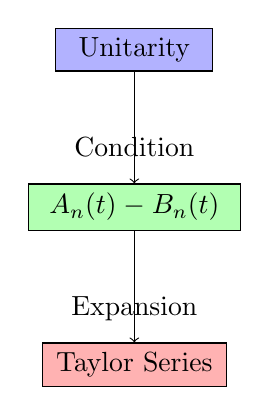
\begin{tikzpicture}[node distance=2cm]
    % Nodes
    \node (unitarity) [rectangle, draw, fill=blue!30, text width=5em, align=center] {Unitarity};
    \node (operators) [below of=unitarity, rectangle, draw, fill=green!30, text width=7em, align=center] {$A_n(t) - B_n(t)$};
    \node (series) [below of=operators, rectangle, draw, fill=red!30, text width=6em, align=center] {Taylor Series};
    
    % Arrows
    \draw [->] (unitarity.south) -- node[anchor=north] {Condition} (operators.north);
    \draw [->] (operators.south) -- node[anchor=north] {Expansion} (series.north);
\end{tikzpicture}

This diagram shows the relationship between the unitarity condition, the difference between two operators, and their Taylor series expansion. You can further customize the nodes and arrows to better fit your specific needs.

If you have more detailed equations or additional components to include, feel free to provide more information, and